% MeanFlow StormCast -- autoregressive inference (1-2 NFE) workflow.
% Notation matches the thesis formula deck (X_{t-1} HighRes state,
% M_t = F_xi(...) regression mean, c_t = concat(X_{t-1},M_t,I)).
\documentclass[border=14pt]{standalone}
% Shared MeanFlow-StormCast workflow style.
% Palette = thesis viridis convention (mirrors make_method_figures.py /
% build_formulas.py): borders at viridis ramp positions, fills tinted to white.
\usepackage{amsmath,amssymb,bm}
\usepackage{xcolor}
\usepackage{tikz}
\usetikzlibrary{positioning,arrows.meta,calc,fit,backgrounds,shapes.geometric}

% --- viridis-sampled palette (border / light fill) -------------------------
\definecolor{cFrozen}{HTML}{481D6F}\definecolor{cFrozenF}{HTML}{EDE8F1} % frozen nets
\definecolor{cSamp}{HTML}{355F8D}\definecolor{cSampF}{HTML}{EBEFF4}     % flow-space / sampler
\definecolor{cFlow}{HTML}{287D8E}\definecolor{cFlowF}{HTML}{E9F2F4}     % trained MeanFlow net
\definecolor{cLoss}{HTML}{1E9C89}\definecolor{cLossF}{HTML}{E9F5F3}     % loss terms
\definecolor{cOut}{HTML}{26AD81}\definecolor{cOutF}{HTML}{E9F7F2}       % composition / output
\definecolor{cData}{HTML}{737373}\definecolor{cDataF}{HTML}{F1F1F1}     % data / tensors
\definecolor{cEdge}{HTML}{5A5A5A}

\tikzset{
  base/.style   ={rounded corners=3pt, draw, line width=0.9pt, align=center,
                  inner sep=5pt, font=\small, text=black!88},
  data/.style   ={base, draw=cData,   fill=cDataF},
  frozen/.style ={base, draw=cFrozen, fill=cFrozenF},
  trained/.style={base, draw=cFlow,   fill=cFlowF},
  sampler/.style={base, draw=cSamp,   fill=cSampF},
  loss/.style   ={base, draw=cLoss,   fill=cLossF},
  output/.style ={base, draw=cOut,    fill=cOutF},
  total/.style  ={base, draw=black!80, fill=black!7, line width=1.1pt},
  flow/.style   ={-{Stealth[length=2.4mm]}, line width=0.9pt, draw=cEdge},
  thin flow/.style={-{Stealth[length=2.0mm]}, line width=0.7pt, draw=cData},
  feedback/.style={-{Stealth[length=2.4mm]}, line width=0.9pt, draw=cData,
                  dashed, dash pattern=on 4pt off 3pt},
  emaedge/.style={-{Stealth[length=2.2mm]}, line width=0.8pt, draw=cData,
                  dashed, dash pattern=on 3pt off 2.5pt},
  container/.style={rounded corners=6pt, draw=black!35, line width=0.8pt,
                  dashed, dash pattern=on 3pt off 2.5pt, fill=black!2,
                  inner sep=8pt},
  ttl/.style    ={font=\bfseries\large, text=black!85},
  sub/.style    ={font=\itshape\footnotesize, text=black!55},
  lg/.style     ={font=\scriptsize, text=black!60},
}

% legend swatch helper
\newcommand{\swatch}[2]{%
  \tikz[baseline=-0.5ex]\node[rounded corners=1.5pt, draw=#1, fill=#1!12,
    line width=0.9pt, minimum width=3.4mm, minimum height=2.6mm, inner sep=0]{};\;#2}

\begin{document}
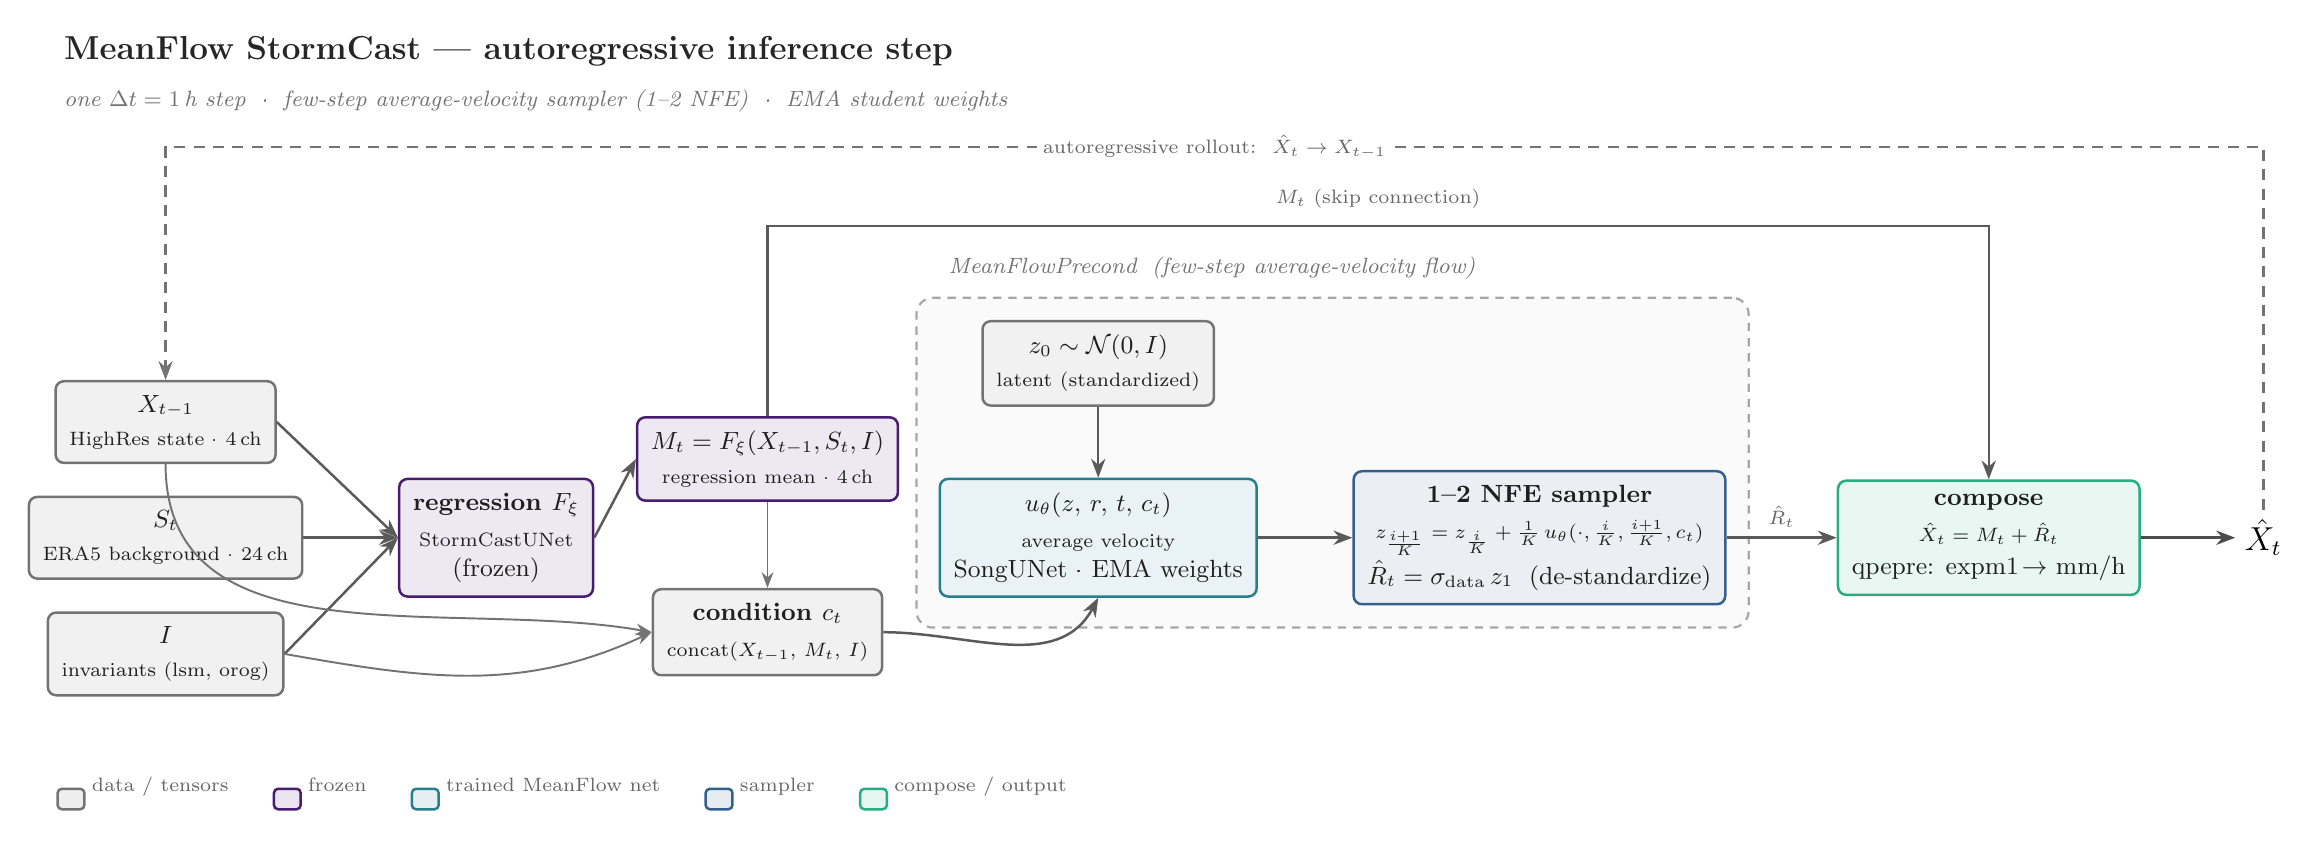
\begin{tikzpicture}[node distance=10mm]

  % ===== pipeline (anchored at the inputs; title + lanes placed afterwards) =====
  % ---- inputs (stacked) ----
  \node[data] (xprev) at (0,0)
    {$X_{t-1}$\\[1pt]\scriptsize HighRes state · 4\,ch};
  \node[data, below=4mm of xprev] (st)
    {$S_t$\\[1pt]\scriptsize ERA5 background · 24\,ch};
  \node[data, below=4mm of st] (inv)
    {$I$\\[1pt]\scriptsize invariants (lsm, orog)};

  % ---- frozen regression ----
  \node[frozen, right=12mm of st] (reg)
    {\textbf{regression $F_\xi$}\\[2pt]\scriptsize StormCastUNet\\(frozen)};

  % ---- regression mean + conditioning bundle ----
  \node[frozen] (mt) at ($(reg.east)+(22mm,10mm)$)
    {$M_t = F_\xi(X_{t-1},S_t,I)$\\[1pt]\scriptsize regression mean · 4\,ch};
  \node[data] (cond) at ($(reg.east)+(22mm,-12mm)$)
    {\textbf{condition $c_t$}\\[2pt]\scriptsize $\mathrm{concat}(X_{t-1},\,M_t,\,I)$};

  % ---- MeanFlow precond block: noise + average-velocity net + sampler ----
  \node[trained] (uth) at ($(reg.east)+(64mm,0mm)$)
    {\textbf{$u_\theta(z,\,r,\,t,\,c_t)$}\\[2pt]\scriptsize average velocity\\SongUNet · EMA weights};
  \node[data, above=9mm of uth] (noise)
    {$z_0\sim\mathcal N(0,I)$\\[1pt]\scriptsize latent (standardized)};
  \node[sampler, right=12mm of uth] (samp)
    {\textbf{1--2 NFE sampler}\\[2pt]\scriptsize $z_{\frac{i+1}{K}}=z_{\frac{i}{K}}+\frac1K\,u_\theta(\cdot,\tfrac{i}{K},\tfrac{i+1}{K},c_t)$\\[1pt]$\hat R_t=\sigma_{\mathrm{data}}\,z_1$ \;(de-standardize)};

  \begin{scope}[on background layer]
    \node[container, fit=(noise)(uth)(samp)] (box) {};
  \end{scope}

  % ---- compose + output ----
  \node[output, right=14mm of samp] (compose)
    {\textbf{compose}\\[2pt]\scriptsize $\hat X_t = M_t + \hat R_t$\\[1pt]qpepre: $\mathrm{expm1}\!\to$ mm/h};
  \node[font=\large\bfseries, right=12mm of compose] (out) {$\hat X_t$};

  % ===== pipeline edges =====
  \draw[flow] (xprev.east) -- (reg.west);
  \draw[flow] (st.east) -- (reg.west);
  \draw[flow] (inv.east) -- (reg.west);
  \draw[flow] (reg.east) -- (mt.west);
  % conditioning bundle = concat(X_{t-1}, M_t, I)
  \draw[thin flow] (mt.south) -- (cond.north);
  \draw[thin flow] (xprev.south) to[out=-90,in=170] (cond.west);
  \draw[thin flow] (inv.east) to[out=-10,in=205] (cond.west);
  % into the MeanFlow block
  \draw[flow] (cond.east) to[out=0,in=-118] (uth.south);
  \draw[flow] (noise.south) -- (uth.north);
  \draw[flow] (uth.east) -- (samp.west);
  % residual into compose
  \draw[flow] (samp.east) -- (compose.west) node[midway,above,lg]{$\hat R_t$};
  \draw[flow, line width=1.1pt, draw=black!70] (compose.east) -- (out.west);

  % ===== top lanes (relative to the container, so they always clear it) =====
  \coordinate (skL) at ($(box.north)+(0,9mm)$);    % M_t skip lane
  \coordinate (fbL) at ($(box.north)+(0,19mm)$);   % autoregressive feedback lane

  % M_t skip connection: regression mean is added back at compose
  \draw[flow] (mt.north) -- (mt.north |- skL) -- (compose.north |- skL) -- (compose.north);
  \node[lg, anchor=south] at ($(mt.north |- skL)!0.5!(compose.north |- skL)+(0,1mm)$)
    {$M_t$ (skip connection)};

  % container label, sitting just above the box top-left, below the skip lane
  \node[sub, anchor=south west] at ($(box.north west)+(3mm,1mm)$)
    {MeanFlowPrecond \;(few-step average-velocity flow)};

  % autoregressive feedback
  \draw[feedback] (out.north) -- (out.north |- fbL) -- (xprev.north |- fbL) -- (xprev.north);
  \node[lg, fill=white, inner sep=2pt]
    at ($(xprev.north |- fbL)!0.5!(out.north |- fbL)$)
    {autoregressive rollout:\; $\hat X_t \rightarrow X_{t-1}$};

  % ===== title + subtitle (placed above all lanes) =====
  \node[ttl, anchor=south west] (title) at ($(xprev.north west |- fbL)+(0,9mm)$)
    {MeanFlow StormCast --- autoregressive inference step};
  \node[sub, anchor=north west] at ($(title.south west)+(0,-0.5mm)$)
    {one $\Delta t=1$\,h step \;·\; few-step average-velocity sampler (1--2 NFE) \;·\; EMA student weights};

  % ===== legend =====
  \node[lg, anchor=north west] at ($(inv.south west)+(0,-9mm)$)
    {\swatch{cData}{data / tensors}\qquad
     \swatch{cFrozen}{frozen}\qquad
     \swatch{cFlow}{trained MeanFlow net}\qquad
     \swatch{cSamp}{sampler}\qquad
     \swatch{cOut}{compose / output}};

\end{tikzpicture}
\end{document}
